\documentclass[12pt]{article}

\usepackage{tikz} % картинки в tikz
\usepackage{microtype} % свешивание пунктуации

\usepackage{array} % для столбцов фиксированной ширины

\usepackage{indentfirst} % отступ в первом параграфе

\usepackage{sectsty} % для центрирования названий частей
\allsectionsfont{\centering}

\usepackage{amsmath, amssymb, amsthm} % куча стандартных математических плюшек

\usepackage{amsfonts}

\usepackage{graphicx}

\usepackage{comment}

\usepackage[top=2cm, left=1.2cm, right=1.2cm, bottom=2cm]{geometry} % размер текста на странице

\usepackage{lastpage} % чтобы узнать номер последней страницы

\usepackage{enumitem} % дополнительные плюшки для списков
%  например \begin{enumerate}[resume] позволяет продолжить нумерацию в новом списке
% \usepackage{caption}

\usepackage{physics}

\usepackage{hyperref} % гиперссылки

\usepackage{multicol} % текст в несколько столбцов

\usepackage{url}

\usepackage{fancyhdr} % весёлые колонтитулы


\usepackage{todonotes} % для вставки в документ заметок о том, что осталось сделать
% \todo{Здесь надо коэффициенты исправить}
% \missingfigure{Здесь будет Последний день Помпеи}
% \listoftodos - печатает все поставленные \todo'шки


% более красивые таблицы
\usepackage{booktabs}
% заповеди из докупентации:
% 1. Не используйте вертикальные линни
% 2. Не используйте двойные линии
% 3. Единицы измерения - в шапку таблицы
% 4. Не сокращайте .1 вместо 0.1
% 5. Повторяющееся значение повторяйте, а не говорите "то же"



\usepackage{fontspec}
\usepackage{polyglossia}

\setmainlanguage{english}
\setotherlanguages{russian}

% download "Linux Libertine" fonts:
% http://www.linuxlibertine.org/index.php?id=91&L=1
\setmainfont{Linux Libertine O} % or Helvetica, Arial, Cambria
% why do we need \newfontfamily:
% http://tex.stackexchange.com/questions/91507/
\newfontfamily{\cyrillicfonttt}{Linux Libertine O}

\AddEnumerateCounter{\asbuk}{\russian@alph}{щ} % для списков с русскими буквами
% \setlist[enumerate, 2]{label=\asbuk*),ref=\asbuk*}


\let\P\relax
\DeclareMathOperator{\P}{\mathbb{P}}
\DeclareMathOperator{\plim}{plim}
\DeclareMathOperator{\E}{\mathbb{E}}
\newcommand{\cN}{\mathcal{N}}
\DeclareMathOperator{\Var}{\mathbb{V}ar}
\DeclareMathOperator{\Cov}{\mathbb{C}ov}
\DeclareMathOperator{\Corr}{\mathbb{C}orr}




\lhead{Олимпиада по теории вероятностей и статистике}
\rhead{2021-04-19, 18:10, R205}
\cfoot{\thepage} 

% версия для гостей ковидария (скрыты решения):
% \excludecomment{solution}
% версия для главврачей (открыты решения):
\newenvironment{solution}{}{}

\usepackage{epigraph}
\setlength\epigraphwidth{.6\textwidth}
\setlength\epigraphrule{0pt}


\title{Один день в сумасшедшем ковидарии}
\date{}

% побег из ковидария или дистант в сумасшедшем доме

\begin{document}
	\maketitle

\section*{Правила}

Запаситесь арбидолом и галоперидолом! Ваша задача — пережить один день, состоящий из трёх фаз лечения в сумасшедшем ковидарии.

\begin{center}
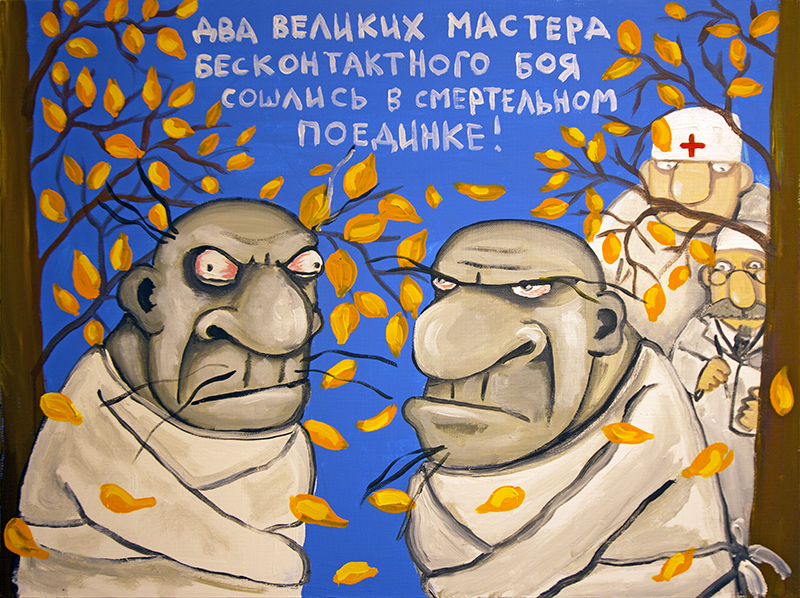
\includegraphics[scale=4]{images/lozhkin.jpg}
\end{center}

Не бойтесь трудностей и не хватайтесь за больные головы, 
ведь у каждой палаты будет свой дежурный врач из числа смелых ассистентов. В каждой палате находится пять гостей. 

Игра начинается с первого этапа утренних невероятных процедур, и гости каждой палаты совместно решают задачи по теории вероятностей. 

Первый этап начнётся 19 апреля в 18:10 в  R205. Но это не точно. 

Главврач любит проводить дуэли между гостями. 
Если он обратит свой взор на палату, то 
один гость палаты уходит в дуэльную процедурную, 
где сражается один на один с соперником из другой палаты. 
В дуэли выигрывает тот, кто первым правильно решит задачу. 
В случае неправильного ответа обоими участниками, дуэльный санитар выбирает победителя по более точному решению.

На втором этапе гостей ковидария ждут вечерние статистические процедуры. В остальном правила второго этапа такие же, как у первого. 

Ночью присмотр в сумасшедшем ковидарии ослабевает и гости предаются азартным играм и оргиям третьего тура олимпиады. 

Регистрация гостей палат сумасшедшего ковидария открыта до 18:18 воскресенья 18 апреля по ссылке \url{https://forms.gle/T41tKCr7D29yPLWo9}.

Гости в самых удачных костюмах получают дополнительные баллы :)
По итогам олимпиады гостей ждут невероятные и статистически значимые призы. На оценку по курсу теории вероятностей или статистики результаты олимпиады не влияют!

На олимпиаде мы ждём всех: как и ИП, как и БП, главное — быть бесстрашным и готовым к любым сложностям!


\begin{comment}
\newpage
\section*{Правила для дежурных врачей}

% Третий игровой тур — перуда (пока это секрет играющих).
Продолжительность задачных туров: 60 минут.
Перерывы — по 10 минут. Игровой тур — 40 минут. 
% всё равно что-то пойдёт не так и мы закончим позже :)
Начало: 18:10. 

В каждой палате 5 человек. Если вдруг спрашивают, можно ли четыре, отвечаем, что можно. Больше — не нужно, меньше четырёх, тоже не нужно. 

Число попыток сдачи задач основной части: без ограничений. 
Последующие попытки сдачи не штрафуются. 



Идеи:

Аскорбиновая кислота. Раздавать со словами «хорошо штырит» или «кислотные» командам, которые верно решают задачи. Упаковочку заклеить словами галоперидол и т.п. 

\end{comment}



\newpage
\section*{Утренние вероятностные процедуры}

\epigraph{-- Ничего не поделаешь, — возразил Кот. — Все мы здесь не в своем уме — и ты, и я! \\
-- Откуда вы знаете, что я не в своем уме? — спросила Алиса. \\
-- Конечно, не в своем, — ответил Кот. — Иначе как бы ты здесь оказалась?}{\textit{Алиса в стране чудес}}


\begin{enumerate}
    
    \item В группе пациентов, поступивших сегодня, есть как больные, так 
и здоровые. Из всех $35$ поступивших пациентов $10$ заражены. Одна палата вмещает $5$ человек. 

    \begin{enumerate}
    \item (2 балла) Какова вероятность, что Илон Маск (один из поступивших пациентов) попадет в палату со всеми здоровыми?    
    
    \item (3 балла) Какова вероятность того, что Илон Маск и Грета Тунберг (два поступивших пациента) попадут в одну палату?
    % \item (3 балла) Какова вероятность, что заразятся все?
   \end{enumerate}
    
\begin{solution}
    \[
    C_{25}^4/C_{35}^4 \approx 0.24
    \]
    \[
    4/34=2/17
    \]
\end{solution}
    
    
    \item (5 баллов) Вася и Петя каждый день принимают таблетки, чтобы вылечиться от ковида. Каждая таблетка равновероятно может оказаться арбидолом или галоперидолом. Вася принимал таблетки в течение $100$ дней, а Петя в течение $101$ дня. 
    
    Найдите вероятность того, что Петя съест больше таблеток арбидола, чем Вася. 

\begin{solution}
Ответ: $0.5$
\end{solution}    
    
    
    \item (5 баллов) Правительство хочет опробовать новую вакцину от короны «Чу-вак\footnote{Чуваки-авторы вакцины никак не аффилированы с центром имени Чумакова!}». Доля пациентов $Z$, на которых будет опробована вакцина, определяется странным образом. Сначала медсестра Анатолий генерирует случайную величину $X$ из распределения с функцией распределения $F_X(\cdot)$, а затем вычисляет значение $Z=F^{-1}_X(X)$. Найдите $\P\{Z > e^{-1}\}$.
    
\begin{solution}
%$Z \sim U[0, 1] \Rightarrow$ искомая вероятность равна $1-e^{-1}$

Правильный ответ $1-F(F(e^{-1}))$
\end{solution}
    
    
    \item (10 баллов) Совместная плотность случайных величин $X, Y, Z$ выглядит следующим образом:
    \begin{equation}
    p(x, y, z)= \begin{cases}
    \cfrac{6}{(1+x+y+z)^4} &  \text{при}\; x^2+y^2+z^2 > 0,\\
    \;\;\;\;\;\;\;\;\;\;\; 0  & \text{иначе}
    \end{cases}
    \end{equation}
    Требуется найти плотность случайной величины $S=X+Y+Z$. Hint: попробуйте через дифференциальные формы (или интегралом для самых брутальных)
    
\begin{solution}
Нужно рассмотреть совместно распределение $R=X/(X+Y+Z), T=Z/(X+Y+Z), S=X+Y+Z$.
Ответ: $p_S(s) =  \frac{3s^2}{(1+s)^4}$

\end{solution}

    
    \item (10 баллов) Чтобы получить дополнительную дозу морфина санитары предлагают вам сыграть в игру. Санитар держит за спиной три пробирки и каждый раз выдает вам одну равновероятно. Выдав вам эту пробирку, он добавляет себе за спину точно такую же, так что в каждом раунде за спиной у него всегда оказывается три пробирки, в двух из которых вода, а в оставшейся капля морфина. 
    
    Игра продолжается до тех пор, пока не попадется третья пробирка с морфином. После каждой пробирки с морфином вы можете прекратить игру и забрать столько миллилитров морфина, сколько раундов потребовалось, чтобы попалась пробирка с ним (не считая предыдущую пробирку с морфином, если она была, но считая текущую). Как следует играть, чтобы математическое ожидание выигрыша миллилитров морфина было максимально возможным, и чему оно равно?  
    
\begin{solution}
    Предположим, что мы уже продолжаем игру после первого герба. Следует остановиться на втором гербе, если $\xi_2 \geq E\xi_3 = 3$, и продолжить игру в противном случае. При этом наш средний выигрыш равен $\frac{35}{9}$. Это число меньше 4, поэтому на первом шаге нам нужно остановиться, если $\xi_1 \geq 4$, и продолжить игру в противном случае. При этом наш средний выигрыш равен 4.51
    
    
\end{solution}
    
    
    % http://new.math.msu.su/department/probab/os/olimpia/olsol14talk.pdf задача 5
    
    \item (10 баллов) Илон Маск разработал новый тест от короны. Он никогда не ошибается. Таких тестов в Лепрозории очень мало. Чтобы сэкономить, санитары решили действовать следующим образом: 
    
    \begin{itemize} 
        \item всех людей разбивают на группы по $k$ человек;
        \item каждая группа сдаёт свою слюну в общую пробирку
        \item если тест показывает, что в пробирке нет вируса, все $k$ человек объявляются здоровыми
        \item если тест показывет, что вирус есть, все $k$ человек сдают индивидуальные тесты
    \end{itemize}
    
    Человек заражается короной с довольно низкой вероятностью $p$. Всего в Лепрозории $n$ человек. На сколько групп нужно разбить людей, чтобы сэкономить как можо больше тестов? Сколько, в среднем, тестов будет потрачено? 
    
    \textbf{Hint:} Для простоты можно считать, что $n$ всегда делится на $k$. Перед тем, как взять производную от математического ожидания числа проверок, воспользуйтесь разложением в ряд Тэйлора: $(1 - p)^x \approx 1 - p \cdot x$. Это можно сделать, если мы предполагаем, что вероятность заболеть, $p$, очень маленькая.  
    
\begin{solution} 
    \begin{equation*}
        X_j = \begin{cases} 
        1, \text{ если все здоровы }, (1 - p)^k \\
        k + 1, \text{ если есть больные }, 1 - (1 - p)^k.
        \end{cases}
    \end{equation*} 
    
    Получается, что всего мы сделаем $Z$ проверок:
    
    $$
    Z = X_1 + \ldots + X_{\frac{n}{k}}.
    $$ 
    
    Наша задача минимизировать среднее число проверок, выбрав оптимальное число групп, то есть
    
    \begin{multline*}
        \mathbb{E}(Z) = \mathbb{E}(X_1 + \ldots + X_{\frac{n}{k}}) = \mathbb{E}(X_1) + \ldots +  \mathbb{E}(X_{\frac{n}{k}}) = \\ =\frac{n}{k} \cdot \mathbb{E}(X_1) = \frac{n}{k} \cdot \left[1 \cdot (1-p)^k + (k+1) \cdot (1 - (1 - p)^k) \right] \to \min_k 
    \end{multline*}

    \begin{equation*} 
    \begin{aligned}
    &\mathbb{E}(Z) = n \cdot \left[1 + \frac{1}{k} - (1-p)^k \right] \to \min_k \\
    &\mathbb{E}(Z) \approx n \cdot \left[1 + \frac{1}{k} - 1 + p \cdot k \right] \to \min_k
    \end{aligned}
    \end{equation*}
    
    Теперь берём производную и решаем уравнение: 
    
    $$
    - \frac{1}{k^2} + p = 0 \quad \Rightarrow \quad \hat k = \frac{1}{\sqrt{p}}
    $$
\end{solution} 

    \item При полевых испытаниях Билл Гейтс выяснил, что, когда нет никаких негативных факторов, его чипы работают бесперебойно с вероятностью $0.99$. При морозах вероятность работоспособности чипа равна $0.95$. Если человек надевает шапочку из фольги, чип работает с вероятностью $0.9$. Если человек надевает шапочку из фольги в мороз, чип работает с вероятностью $0.8$. 

    В России морозы наступают с вероятностью $0.2$, а шапочку из фольги надевают с вероятностью $0.1$. 

    \begin{itemize}
    \item (2 балла) Какова вероятность того, что чип отключится, если морозы и ношениче шапочки из фольги не зависят друг от друга?
    
    \item (3 балла) В каком диапазоне лежит вероятность того, что отключит чип, если морозы и ношение шапочки зависят друг от друга? 
    \end{itemize} 
    
\begin{solution}
\[P(A) = 0.9 \cdot 0.8 \cdot 0.01 + 0.9 \cdot 0.2 \cdot 0.05 + 0.1 \cdot 0.8 \cdot 0.1 + 0.1 \cdot 0.2 \cdot 0.2 = 0.028\]
    
Берём за $x$ любую условную вероятность. Например $P(B_2 \mid B_1)$, где $B_1$ - наступил мороз, $B_2$ - чипированный носит шапочку. Выражаем все вероятности через неё
    
\[
0.1 \cdot x \cdot 0.2 + 0.1 \cdot (1-x) \cdot 0.1 + \\ + 0.9 \cdot \frac{0.2 - 0.1x}{0.9} \cdot 0.05 + 0.9 \cdot (1 - \frac{0.2 - 0.1x}{0.9}) \cdot 0.01.
\]

Подставляем вместо $x$ сначала $0$, затем $1$, получаем диапазон от $0.027$ до $0.033$
\end{solution}

     \item (5 баллов) Для борьбы с коронавирусной инфекцией чрезвычайно полезно знать функцию плотности для распределения Лапласа:
    $$p(x) = \cfrac{\alpha}{2}e^{-\alpha|x-\beta|}$$
    Медсестра Саша хочет найти дифференциальную энтропию данного распределения, которая считается следующим образом:
    $$H(X) = - \int \limits_{\mathbb{R}} p(x)\log p(x) dx$$
    
    Помогите Саше!
    
\begin{solution}
Ответ: $1-\log(\alpha/2)$
\end{solution}
    
    \item (10 баллов) Как-то собрались Крош, Ёжик и Нюша загадать стороны мнимого параллелепипеда. Начинает Крош, и он загадывает $X \sim U[1, 2]$. Затем Ёжик, как великий мимикрятор, загадывает число не больше, чем число Кроша, то есть $Y \sim U[1, X]$. Так же поступает далее Нюша: $Z \sim U[1, Y]$. Чему равен ожидаемый объем данного параллелепипеда?
    
\begin{solution}
    Найдем совместную функцию плотности:
    
    $f_{X, Y, Z}(x, y, z) = f_{Z \mid X, Y}(z \mid x, y) \cdot f_{X, Y}(x, y) = f(z \mid y) \cdot f(y \mid x) \cdot f(x) = \frac{1}{(x - 1)(y - 1)}$
    
    Тогда математическое ожидание объема параллелепипеда можно найти, посчитав тройной интеграл:
    
    $\Large \displaystyle \int_1^2 \int_1^x \int_1^y \frac{xyz}{(x-1)(y-1)}\, dz\, dy\, dx = \dots = \frac{20}{9}$
\end{solution}
    
    \item (5 баллов) Игральную кость подбросили n раз. Пусть $X_1$ - число выпадений 1, а $X_2$ - число выпадений 2. 
    
    Чему равна $\Corr{(X_1, X_2})$?
    
\begin{solution}
    С одной стороны, $X_1 + X_2 + X_3 + X_4 + X_5 + X_6 = n$, то есть константа, отсюда:
    
    $\Cov{(X_1, X_1 + \dots + X_6)} = \Cov{(X_1, X_1)} + \Cov{(X_1, X_2)} + \Cov{(X_1, X_3)} + \Cov{(X_1, X_4)} + \Cov{(X_1, X_5)} + \Cov{(X_1, X_6)} = \Cov{(X_1, n)} = 0$
    
    Заметим, что $\Cov(X_1, X_i) \forall i \neq 1$ не зависит от номера i, то есть:
    
    $\Var(X_1) + 5\Cov(X_1, X_2) = 0 \Rightarrow \Cov(X_1, X_2) = -\frac{\Var(X_1)}{5} = -\frac{n \cdot 1/6 \cdot 5/6}{5} = -\frac{n}{36}$
    
    Последний шаг:
    
    $\Corr(X_1, X_2) = \frac{\Cov(X_1, X_2)}{\sqrt{\Var(X_1) \cdot \Var(X_2)}} = \frac{-n / 36}{5n/36} = -\frac{1}{5}$
\end{solution}
    
    \item Как-то санитары и пациенты решили устроить футбольный матч. Ничья возможна. Время ожидания очередного гола не зависит от предыдущих событий матча. Известно, что математическое ожидание общего числа голов в футбольных матчах равно $\ln{20}$. 
    
    \begin{enumerate}
        \item (4 балла) Какова вероятность того, что в итоге будет забито четное количество голов?    
        
        \item (1 балла) Как думаете, для какого класса предназначена данная задача?
    \end{enumerate}
    
    \textit{Hint}: отсутствие памяти ни о чем не говорит?
    
\begin{solution}
    Из условия понятно, что количество голов имеет распределение Пуассона с параметром $\lambda = \ln{20}$. Тогда вероятность забить четное число голов и нечетное число голов:
    
    $p = e^{-\lambda} \cdot (1 + \frac{\lambda^2}{2!} + \frac{\lambda^4}{4!} + \dots)$
    
    $q = e^{-\lambda} \cdot (\frac{\lambda^1}{1!} + \frac{\lambda^3}{3!} + \dots)$
    
    Тогда $p - q = e^{-\lambda} \cdot(1 - \frac{\lambda^1}{1!} + \frac{\lambda^2}{2!} + \dots) = e^{-2\lambda}$
    
    Тогда из данного условия и $p + q = 1$ получаем $p = \frac{1 + e^{-2\lambda}}{2} = \frac{1 + 1/400}{2} = \frac{401}{800}$
    
    Задача для 10 класса.
\end{solution}
    
    \item По вечерам Коши и Буняковский собираются играть в их любимый дартс. Мишень у них была такая, что сектора были неравны, то есть вероятности попасть в разные секторы не равны между собой. Центрального участка на мишени нет (то есть представьте себе криво порезанный пирог, это и есть примерно мишень). Пусть Коши бросил дротик и попал в мишень.
    
    \begin{enumerate}
        \item (9 баллов) Что более вероятно: что Буняковский попадет в этот же сектор, или попадет в следующий по часовой стрелке?
        \item (1 балл) Как думаете, для какого класса данная задача?
    \end{enumerate}
    
\begin{solution}
    Вероятность попасть в тот же сектор:
    
    $p_1^2 + p_2^2 + \dots + p_n^2$
    
    Попасть в соседний сектор:
    
    $p_1 \cdot p_2 + p_2 \cdot p_3 + p_n \cdot p_1$
    
    И можно сравнить либо с помощью неравенства Коши-Буняковского:
    
     $p_1^2 + p_2^2 + \dots + p_n^2 = \sqrt{p_1^2 + p_2^2 + \dots + p_n^2} \cdot \sqrt{p_1^2 + p_2^2 + \dots + p_n^2} \geq p_1 \cdot p_2 + p_2 \cdot p_3 + p_n \cdot p_1$
     
     Так как вероятности неравны, то знак будет строго больше.
     
     Можно через квадраты:
     
     $2(p_1^2 + p_2^2 + \dots + p_n^2) - 2(p_1 \cdot p_2 + p_2 \cdot p_3 + p_n \cdot p_1) = (p_1 - p_2)^2 + (p_2 - p_3)^2 + (p_3 - p_4)^2 + \dots + (p_n - p_1)^2 > 0$
     
     Задача для 9 класса.
\end{solution}
    
    \item Павел в свободное время любит загадывать числа.
    
    \begin{enumerate}
        \item (2 балла) Пусть он равномерно загадывал тысячу цифр $x_1, \dots, x_{1000}$ (от 0 до 9), а затем записал следующую величину $X = 0,x_1 x_2 \dots x_{1000}$. Чему равно математическое ожидание $X$? К чему оно стремится при стремлении количества цифр после запятой к бесконечности?
        \item (3 балла) Теперь Паша решил пойти в ва-банк, и загадать столько цифр, сколько он сможет, но теперь вероятность того, что он загадает цифру $k$, пропорциональна величине $k + 1$. Так же он записывает величину $X = 0,x_1 x_2 \dots x_n$. К чему теперь стремится $\E{X}$?
    \end{enumerate}
    
\begin{solution}
    Запишем число в следующем виде: $X = 0.1^1 \cdot x_1 + 0.1^2 \cdot x_2 + \dots + 0.1^{1000} \cdot x_{1000}$
    
    Математическое ожидание каждой $x_i$ равно 4,5. Тогда:
    
    $\E(X) = 0.45 + 0.045 + 0.0045 + \dots = 0.4999\dots995$ (тут 999 девяток)
    
    Для второго пункта $P(x_i = k) = \frac{k + 1}{55}$. Тогда $\E(x_i) = \sum_{k = 0}^{9} \frac{k^2 + k}{55} = 6$. Тогда $\E{X} = 0.6 + 0.06 + 0.006 + \dots = 0.666\dots66$ (тут n шестерок). Стремится к $\frac{2}{3}$
\end{solution}
    

\end{enumerate}



\newpage
\subsection*{Вероятностные дуэли}




\begin{enumerate}
    \item Ваш отчаявшийся сосед по палате решил повеситься на петле из бинтов. В руке у него зажаты 6 кусочков бинтов так, что их концы выступают сверху и снизу. Верхние концы случайным образом разбиваются на пары и связываются между собой. То же делают и с нижними концами. 
    
    Какова вероятность того, что в результате этой операции все 6 концов окажутся связанными в одну петлю и ему удастся вырваться из жизни?
    
\begin{solution}
    Если верхние концы уже как-то связаны, то число благоприятных исходов связывания нижних концов, очевидно, одно и то же для всех связываний верхних. Поэтому будем считать, что связка верхних фиксирована. Например, считаем, что связаны кусочки номер 1 и 2, номер 3 и 4, номер 5 и 6. Способов связать нижние имеется всего $C_6^2 \cdot C_4^2 = 90$ (на пером шаге выбираем две травинки из шести, на втором две из оставшихся). Вычислим, сколько из этих способов благоприятных. Выбрать первую связываемую пару можно $C_6^2 - 3$ способами (есть только три пары, которые выбирать нельзя). После этого остается 4 травинки, у ровно двух из которых связаны верхние концы. Поэтому на втором шаге нельзя выбирать вместе ни их, ни две остающиеся, значит, имеем 4 способа. Всего получается 48 способов. Ответ: $\frac{8}{15}$.
\end{solution}

    \item Коридор больницы имеет форму треугольника. Буйный пациент равновероятно находится в случайной вершине коридора. Медсестра, которая хочет поставить ему укол, может заглянуть в любую вершину, чтобы проверить, не затаился ли там пациент. После этого пациент случайным образом перебегает в вершину, соседнюю по стороне. Какова вероятность успокоить пациента за не более чем две проверки при оптимальной стратегии?
    
\begin{solution}
$\frac{1}{3} + \frac{1}{2} * \frac{2}{3} = \frac{2}{3}$
\end{solution}
    
    \item Доктор Пуассон кладет вакцину от коронавируса равновероятно в одну из $n=2^r-1$ коробок. Медсестра Бри ищет вакцину следующим образом: проверяет коробку, стоящую посередине, в случае неудачи - уханьский повар подсказывает ей, в какую из двух сторон двигаться, и она второй раз выбирает среднюю коробку с нужной стороны. Это повторяется до тех пор, пока она не найдет вакцину. Найдите выражение для величины $m(r)$, которая равна ожидаемому количеству открытых коробок. Чему будет равен следующий предел: $\lim_{n \to \infty} \frac{\log n}{m(r)}$?
    
\begin{solution}
    Пусть $X$ -- количество открытых коробок. Можно заметить, что $\P\{X=k\} = \cfrac{2^{k-1}}{2^r-1}$. Тогда математическое ожидание считается следующим образом:
    $$
    m(r) = \E X = \sum_{k=1}^{r} \cfrac{k2^{k-1}}{2^r-1} = \cfrac{r2^r}{2^r-1} - 1 
    $$
\end{solution}
    
    \item У Медсестры Саши есть шестипатронный револьер. В него вставлено два патрона подряд. Саша прокручивает револьер и стреляет себе в голову. Она остаётся в живых и отдаёт его первому попавшемуся пациенту. Что выгоднее сделать пациенту: прокрутить барабан или стрелять сразу? С какой вероятностью пациент умрёт в обеих ситуациях?
    
\begin{solution}
    Если прокрутим, $\frac{2}{6}$. Без прокрутки — $\frac{1}{4}$.
\end{solution}
    
    \item Бесконечное количество врачей в конце рабочего дня повесили свои халаты на вешалку, а на следующее утро каждый из них надел случайный халат. Найдите вероятность того, что ни один из них не надел утром тот же халат, в котором был вчера.
    
\begin{solution}
    Ответ: $\lim_{n \to \infty}(1-\frac{1}{n})^{n}=\frac{1}{e}$
\end{solution}

    \item В затылок друг другу выстроились n гостей сумасшедшего ковидария. Понятное дело, более высокие загораживают более низких. Найдите ожидаемое количество людей, которое увидит санитар Николай?
    
\begin{solution}
    Пусть $X_n$ - это количество людей из n, которых видно. Если мы знаем $\E({X_{n - 1}})$, то при добавлении n-го человека с вероятностью $\dfrac{1}{n}$ мы увидим еще одного человека (он окажется самым высоким), а с вероятностью $1 - \dfrac{1}{n}$ математическое ожидание не изменится. Тогда можно записать рекурентное соотношение:
    
    $X_n = \dfrac{1}{n} \cdot (X_{n - 1} + 1) + (1 - \dfrac{1}{n}) \cdot X_{n - 1} = X_{n-1} + \dfrac{1}{n} = \dots = X_1 + \frac{1}{2} + \dots + \frac{1}{n}$
    
    Отсюда же $\E(X_n) = \E(X_1) + \frac{1}{2} + \dots + \frac{1}{n}$. Понятно, что $X_1 = 1$ всегда, отсюда $\E(X_n) = \sum_{k = 1}^n \frac{1}{k} = H_n$
\end{solution}

    \item Имеются два симметричных кубика. Помогите гостю ковидария написать на их гранях некоторые числа, чтобы сумма очков при бросании принимала значения 1, 2, ..., 36 с равными вероятностями.
    
\begin{solution}
    Пример - \{1, 2, 3, 4, 5, 6\}, \{0, 6, 12, 18, 24, 30\}.
\end{solution}

    \item Палату назовем \textit{душной}, если в ней обитает не менее 10 гостей чудного ковидария. Санитары Саша и Глеб задумались, вероятность какого события больше:
    
    A = \{наугад выбранный гость ковидария живет в \textit{душной} палате\}
    
    или
    
    B = \{наугад выбранная палата — \textit{душная}\}.
    
    Помогите им с данной дилеммой.
    
\begin{solution}
    Вероятность события A больше.
\end{solution}
    
    \item Санитары больницы разыскивают пациента, не желающего чипироваться. Вероятность того, что он находится в одной из восьми палат ковидария, составляет $0.8$. Санитары осмотрели семь палат, но ни в одной из них буйный субъект обнаружен не был. С какой вероятностью он будет пойман в восьмой палате?
    
\begin{solution}
     Мысленно добавим к общему числу палат $2$ несуществующие и получим $10$ палат, в каждой из которых пациент окажется с вероятностью $0.1$. Известно, что в $7$ реальных палатах его не обнаружили, а из трех оставшихся реальна только одна. Поэтому там он окажется с вероятностью $\frac{1}{3}$.
\end{solution}

    \item Пусть $\xi$ и $\eta$ -- две случайные величины. Известно, что $\P\{\eta>x\} = \P\{\eta<-x\}, \forall x \in \mathbb{R}$ и что $\P\{\eta = 0\} = 0$. Найдите вероятность того, что функция
    
    $$f(t) = \xi^2 + t(\eta + t)$$
    
    монотонно возрастает при $t \geq 0$.
    
\begin{solution}
    Ответ: $\frac{1}{2}$.
\end{solution}
    
    \item Доктор Коши Буняковский подбросил игральный кубик три раза. Какова вероятность того, что полученные числа могут быть длинами сторон некоторого треугольника?

\begin{solution}
    Пусть $B_{i,k}$ -- событие, заключающееся в том, что на $i$-м броске выпало $k$ очков, а в двух остальных бросках сумма не больше $k$. Тогда $\sum\limits_{i}\sum\limits_{k}B_{i,k}$ есть событие, обратное к искомому. Так как количество натуральных решений неравенства $x+y \leq k$ равно $1+2+ \ldots + (k-1) = \frac{k(k-1)}{2}$, то $\P\{B_{i,k}\} = \frac{1}{6} \cdot \frac{k(k-1)}{2 \cdot 6^2}$. Тогда
    
    $$\P\{A\} = 1 - \sum\limits_{i=1}^3\sum\limits_{k=2}^6\P\{B_{i,k}\} = \frac{37}{72}$$
    
    Ответ: $\frac{37}{72}$.
\end{solution}    

    \item Как-то Яша Бернулли решил подбросить игральную кость шесть раз. Чему равно математическое ожидание числа различных выпавших граней? 
    
\begin{solution}
    Ответ: $6 \cdot \left(1 - (\frac{5}{6})^6\right)$
\end{solution}
    
    \item Одному пациенту приснился сон, в котором $n$ Слоукингов лезли вверх по веревке во время грозы. С вероятностью $0 < p < 1$ каждый Слоукинг, независимо от других, может испугаться грозы и свалиться, попутно сшибая всех Слоукингов, которые находятся ниже. Чему равна вероятность того, что упадет ровно k Слоукингов?
    
\begin{solution}
    Ответ: $p \cdot (1 - p)^{n - k}$
\end{solution}
    
    \item Доктор Малахов для обхода заходит в случайную палату. Всего в сумасшедшем ковидарии $n$ палат. 
    
    Чему равна дисперсия номера случайной палаты?
    
    Hint: лишь безумцы пробуют прибавить к номеру палаты случайную величину, равномерную на отрезке $[0;1]$.
    
\begin{solution}
    \[
    (n^2 - 1)/12
    \]
\end{solution}
    
    
\end{enumerate}


\newpage
\section*{Вечерние статистические процедуры}

\begin{enumerate}

    \item (5 баллов) Утром главврач Малахов обходит две случыйные палаты ковидария.
Он и сам безумен, а потому может посетить одну и ту же палату два раза. Все палаты занумерованы от 1 до $n$.  
    
    Главврач Малахов заметил, что разница номеров посещённых палат равна $10$ по модулю.
    
    Оцените $n$ методом максимального правдоподобия.
\begin{solution}
    \[
    \max 2(n-10) / n^2 
    \]
    \[
    \hat n = 20
    \]
\end{solution}
    
    
    \item Утром главврач Малахов обходит две случыйные палаты ковидария.
Он и сам безумен, а потому может посетить одну и ту же палату два раза. Все палаты занумерованы от 1 до $n$.  
    
    Главврач Малахов заметил, что квадрат разницы номеров посещённых палат равен $100$ по модулю.
    
    Оцените $n$ методом моментов.
    
\begin{solution}
    \[
    100 = \frac{\hat n^2 - 1}{6}
    \]
    \[
    \hat n = \sqrt{601} \approx 24.52
    \]
\end{solution}


        \item
        
        Особо буйная пациентка Тукова каждый день получает $n$ таблеток галоперидола и пытается выкинуть их в форточку. Под её окном расположена урна, так что она старается каждый раз попасть в неё, чтобы таблетки на земле не заметили санитары. Тукова бросает таблетки по одной и в среднем попадает. Математическое ожидание ошибки броска в сантиметрах (перелёты или недолёты) равно нулю. Для простоты считаем, что вправо или влево Тукова не ошибается. Однако с каждым броском вероятность появления санитара в палате увеличивается и пациентка торопится, так что дисперсия ошибки броска равна $k \sigma^2$, где $k$--номер броска.
        
        Вчера санитары просмотрели записи с камер и установили ошибки Туковой за последний день (в соответствии с порядком бросков):
        
        $$9, -11, 0, 30, -67, -41, 37, 55, 56, -105$$
        
    \begin{enumerate}
    \item (3 балла) Предложите несмещенную оценку для $\sigma^2$, докажите ее несмещенность. 
    \item (2 балла) Постройте $90\%$ доверительный интервал для параметра. Какой предпосылкой о распределении вы пользовались? (Достаточно формулы)
    \end{enumerate}

\begin{solution}
Наблюдения следует поделить на $\sqrt{k}$
\end{solution}
    
    
    
    \item Бернард и Линайна украли у главврача стетоскоп и несколько баночек с таблетками. Прямо сейчас они сидят под столом и пытаются взвешивать таблетки на стетоскопе. Вес таблеток имеет какое-то распределение с математическим ожиданием $\mu$ и дисперсией $\sigma^2$. Всего в баночке $100$ таблеток. Пациенты хотят оценить средний вес таблетки в конкретной баночке.

    \begin{enumerate}
    \item (2 балла) Бернард достаёт таблетку, взвешивает её, а затем кидает назад в баночку. Он так делает $n < 100$ раз, а затем считает среднее. Найдите $\Cov(X_1, X_2)$, $\E(\bar x)$ и $\Var(\bar x)$.
    \item (3 балла) Линайна достаёт таблетку, взвешивает её, а затем съедает. Она так делает $n < 100$ раз, а затем тоже считает среднее. Найдите $\Cov(X_1, X_2)$, $\E(\bar x)$ и $\Var(\bar x)$. Чья оценка математического ожидания обладает меньшей дисперсией? 
    \end{enumerate}

\begin{solution} 
Для Бернарда: $\E(\bar x) = \mu$, $\Cov(X_1, X_2) = 0$, $\Var(\bar x) = \frac{\sigma^2}{n}$.

Для Линайны: $\E(\bar x) = \mu$, $\Cov(X_1, X_2) = - \frac{\sigma^2}{99}$, $\Var(\bar x) = \frac{n \cdot \sigma^2 - 2 \cdot C_n^2 \cdot \Cov(X_1, X_2)}{n^2}$.

При поиске ковариации пользуемся тем, что $\Cov(X_1, X_1 + \ldots + X_{100}) = 0$.
\end{solution} 

    \item (5 баллов) Чужестранец встречает толпу энергичных ассистентов, которым лишь бы загрузить студентов задачами. Каждую минуту чужестранец решает одну задачу, тем самым изгоняя одного ассистента. Вероятность того, что появится s новых ассистентов (где s = $0, 1, 2$) на месте изгнанного, равна 
    
    \[p_s = \frac{x^s}{(1 + x + x^2)}\]
    
    Здесь $x > 0$ - некий параметр, показывающий живучесть ассистентов. Чужестранец записывал в течение первых 10 минут количество новых ассистентов, получив выборку:
    
    $\{0, 1, 1, 0, 2, 2, 1, 0, 1, 2\}$
    
    Найдите ML-оценку параметра $x$.
    
\begin{solution}
    Запишем функцию правдоподобия:
    
    $L(x) = \frac{x^{10}}{(1 + x + x^2)^{10}}$
    
    Теперь прологарифмируем:
    
    $l(x) = 10\ln{x} - 10\ln{(1 + x + x^2)}$
    
    Возьмем первую производную:
    
    $l'(x) = \frac{10}{x} - \frac{10(2x + 1)}{1 + x + x^2} = 0$
    
    Можно решить квадратное уравнение: $x^2 + x + 1 = 2x^2 + x$, и получить $x = \pm 1$. Отсюда $x_{ML} = 1$ (проверяется, что максимум, спокойно).
\end{solution}

    \item (10 баллов) Коля решил зачем-то найти ML-оценки для параметров гамма-распределения (зачем, не очень понятно). Для этого он вспоминает функцию плотности гамма распределения:
    
    $f(x) = x^{k - 1} \dfrac{e^{-x / \theta}}{\theta^k \cdot \Gamma{(k)}}$
    
    Помогите ему найти ML-оценки параметров $k$ и $\theta$.
    
    \textbf{Hint:} Николай вспомнил чудесный факт: $\dfrac{\Gamma'{(k)}}{\Gamma{(k)}} \approx \ln{k} - \dfrac{1}{2k}$, он должен вам помочь, так что пользуйтесь.
    
\begin{solution}
  Запишем функцию правдоподобия:
  
  $L = \prod_{i = 1}^n x_i^{k - 1} \cdot \frac{e^{-x_i / \theta}}{\theta^k \Gamma(k)}$
  
  Прологарифмируем:
  
  $l = \ln{L} = (k - 1) \sum \ln{x_i} - \frac{\sum x_i}{\theta} - nk \ln{\theta} - n \ln{\Gamma(k)} \rightarrow \max$
  
  FOC:
  
  $\begin{cases}
  \frac{\partial l}{\partial k} = \sum \ln{x_i} - n\ln{\theta} - n \frac{\Gamma'{(k)}}{\Gamma{(k)}} = 0 \\
  \frac{\partial l}{\partial \theta} = \frac{\sum x_i}{\theta^2} - \frac{nk}{\theta} = 0
  \end{cases}$
  
  Из второго уравнения получаем $\hat{\theta}_{ML} = \frac{\bar{x}}{k}$. Подставим в первое уравнение и заменим логарифмическую производную гаммы-функции:
  
  $\sum \ln{x_i} - n\ln{(\frac{\bar{x}}{k})} - n (\ln{k} - \frac{1}{2k}) = \sum \ln{x_i} - n\ln{\bar{x}} + \frac{n}{2k} = 0$
  
  Поделим все на n:
  
   $\bar{\ln{x}} - \ln{\bar{x}} + \frac{1}{2k} = 0$
   
   Отсюда $\hat{k}_{ML} = \frac{1}{2 \cdot(\bar{\ln{x}} - \ln{\bar{x}})}$ 
   
   Тогда $\hat{\theta}_{ML} = 2\bar{x}(\bar{\ln{x}} - \ln{\bar{x}})$
\end{solution}
    
    \item (10 баллов) Коридор ковидария имеет форму прямоугольного треугольника с гипотенузой, равной $3$. Найдите наименьшее возможное стандартное отклонение сторон этого треугольника. При каких значениях длин катетов оно достигается? 

\begin{solution}   
    Из неравенства средних:
    
    $$a+b \leq 2\sqrt{\frac{a^2+b^2}{2}}=2\frac{3}{\sqrt{2}}=3\sqrt{2}.$$
    
    Тогда:
    
    $$\hat{\sigma}^2 \geq 6-(\frac{3\sqrt{2}+3}{3})^2=3-2\sqrt{2}=(\sqrt{2}-1)^2.$$
    
   Следовательно: 
   
   $$\min{\hat{\sigma}}=\sqrt{2}-1 \approx 0.414.$$
   
   Оно достигается при нулевой дисперсии длин катетов, то есть при $a=b=3\sqrt{2}$.
    
    Ответ: $\min{\hat{\sigma}} = \sqrt{2} - 1 \approx 0.414$, $a = b = \frac{3\sqrt{2}}{2}$.
\end{solution}

    \item Обозначим за $U_k$ долю пациентов, которым в день $k$ приснились бобры. $U_1, \ldots, U_n$ -- iid величины из распределения $U[0, 1]$. 
    
    \begin{enumerate}
        \item (4 балла) Найдите распределение $U_{(7)}$.
        \item (1 балл) Как называется данное распределение?
    \end{enumerate} 
    
\begin{solution}
Должно получиться Бета-распределение $B(7, n-6)$ :)
$$p(u)=\cfrac{n!}{(n-1)!(k-1)!}u^{k-1}(1-u)^{n-k}$$
\end{solution}
    
    \item Светофор на пешеходном переходе разрешает переходить дорогу одну минуту, а n минут запрещает. Известно, что среднее время ожидания зеленого света пешеходами равно 1.6 минутам.
    
    \begin{enumerate}
        \item (5 баллов) Найдите оценку для n методом моментов.
        \item (5 баллов) Пусть еще известно, что количество пешеходов равно 300 , а $\hat{\sigma}^2 = 3$.
        
        Постройте 95\%-ый доверительный интервал для n (возьмите критическое значение, равное 2, для упрощения расчетов). 
    \end{enumerate}
    
\begin{solution}

    Посчитаем мат. ожидание времени ожидания. С вероятностью $\frac{1}{n + 1}$ человек придет во время зеленого сигнала и не должен будет знать. С вероятностью $\frac{n}{n + 1}$ он попадет на красный, где время ожидания распределено равномерно, то есть мат. ожидание $\frac{n + 0}{2} = \frac{n}{2}$. Тогда:
    
    $\E(X) = \frac{1}{n + 1} \cdot 0 + \frac{n}{n + 1} \cdot \frac{n}{2}= \frac{n^2}{2n + 2}$
    
    Метод моментов:
    
    $\frac{n^2}{2n + 2} = \bar{X} = 1.6$
    
    Отсюда $n^2 - 2\bar{X}n -2\bar{X} = 0$
    
    Решаем квадратное уравнение, получаем $\hat{n}_{MM} = \bar{X} + \sqrt{(\bar{X})^2 + 2\bar{X}}$
    
    Для нашей задачи $\hat{n} = 4$.
    
    Теперь считаем дисперсию оценки, так как наблюдений много, то достаточно посчитать производную функции в точке:
    
    $g' = 1 + \frac{2\bar{X} + 2}{2 (\sqrt{(\bar{X})^2 + 2\bar{X}})} = \frac{25}{12}$
    
    Тогда 95\%-доверительный интервал (пусть критическое значение 2):
    
    $[4 - 2 \cdot \sqrt{\frac{3 \cdot \frac{25^2}{12^2}}{300}}; 4 + 2 \cdot \sqrt{\frac{3 \cdot \frac{25^2}{12^2}}{300}}]$
    
    $[4 - 2 \cdot \frac{25}{12} \cdot \frac{1}{10}; 4 + 2 \cdot \frac{25}{12} \cdot \frac{1}{10}]$
    
    $[\frac{43}{12}; \frac{53}{12}]$
\end{solution}
    
    
    
    \item (5 баллов) Уровень безумности у трёх случайно выбранных больных равен $-2$, $5$ и $28$.
    
    Известно, что безумность распределена с плотностью 
    \[
    f(x) = 0.5 \lambda \exp(\lambda \abs{x-a}).
    \]
    
    Оцените $a$ (3 балла) и $\lambda$ (2 балла) методом максимального правдоподобия.


\begin{solution}
    \[
    \hat a = Med(-2, 5, 28) = 5
    \]
    \[
    \hat\lambda = \frac{n}{\sum \abs{x_i - \hat a}} = 0.1
    \]
\end{solution}

\end{enumerate}


\newpage

\section*{Статистические дуэли}

\begin{enumerate}
    \item Пусть $X_1, \dots, X_n$ - некоторая случайная выборка с математическим ожиданием, равным $\ln{29}$. 
    
    Помогите Егору распилить $\plim{\dfrac{X_1}{\bar{X}}}$.
    
\begin{solution}
$X_1 / \ln 29$
\end{solution}
    
    \item Пусть $X_1, \dots, X_n$ - некоторая случайная выборка с математическим ожиданием, равным $\ln{29}$. 
    
    Помогите Егору распилить $\plim{\dfrac{X_n}{\sum_{k = 1}^n X_k}}$

\begin{solution}
$0$
\end{solution}

    
    \item Пусть $X_1, \dots, X_n$ - некоторая случайная выборка с математическим ожиданием, равным $\ln{29}$. 
    
    Помогите Егору распилить $\plim{e^{\bar{X}}}$.

\begin{solution}
$29$
\end{solution}


    \item Как изменится выборочная дисперсия от вектора из выборочного среднего, выборочной моды и выборочной медианы, если каждый член исходной выборки уменьшить в 5 раз?

\begin{solution}
Выборочное среднее уменьшилось в 5 раз.

Мода – это варианта с наибольшей частотой. Так как все варианты уменьшились в 5 раз, а частоты остались прежние, мода тоже уменьшится в 5 раз.

Медиана – это варианта в середине ряда. Так как все варианты уменьшились в 5 раз, медиана останется на том же месте в выборке и тоже уменьшится в 5 раз.

Выборочная дисперсия вектора из трех чисел уменьшится в 25 раз.
\end{solution}
   
    \item Первый пациент написал на стене число 1, а потом еще несколько чисел. Как только он записывает число, второй пациент вычисляет медиану имеющегося набора и записывает ее на другую стену. Через какое-то время на второй стене оказались записаны числа: $1; 2; 3; 2.5; 3; 2.5$. Какое число было записано на первой стене четвертым?
    
\begin{solution}
    Ответ: $2$
\end{solution}
   
    \item Получать десерт в столовой могут лишь те пациенты, вес которых не превышает 70 кг. Есть четыре палаты А, Б, В и Г. Все пациенты в этих палатах хотят получать сладкое и просят разрешить им главврача. Он же производит отбор по весу.
    \begin{itemize}
        \item В палате A средний вес пациентов равен 69 кг.
        \item В палате Б медиана веса пациентов равна 69 кг.
        \item В палате В самый тяжелый пациент имеет вес 71 кг.
        \item В палате Г мода веса пациентов равна 65 кг.
    \end{itemize}
В какой палате по крайней мере половина пациентов точно сможет получать десерт?

\begin{solution}
Контрпример для  А: три матроса с ростом  75, 75 и 57 см. Средний вес 69 кг, но двое из трёх не годны. 
Контрпример для В: два пациента с весом 71 кг. Оба не подходят. Команда В тоже не дает ответа на вопрос.
Контрпример для команды Г: пять пациентов с весом 65, 65, 71, 73, 75 кг. Мода равна 65, но трое из пяти не могут служить на лодке.
Рассмотрим команду Б. По определению медианы не меньше половины пациентов имеют вес не больше 69 см. Эти матросы могут служить на подводной лодке. А, возможно, есть еще такие, чей вес ровно 70. Таким образом, заведомо не менее половины пациентов могут получать десерт.
\end{solution}

    \item Во всех корпусах ковидария 100 палат, занумерованных по порядку. Если выкинуть один номер палаты, то медиана оставшихся номеров будет равна 78. Если выкинуть другой номер палаты, то медиана оставшихся будет 66. Найдите медиану всего набора.

\begin{solution}
Расположим числа в порядке возрастания. Если выкинуть число из первой половины ряда (с номером до 50), то медианой оставшихся чисел будет 51-е число ряда. Если выкинуть число из второй половины, то медианой оставшихся чисел станет число с номером 50, но оно не больше чем 51-е число. Таким образом, 50-е число равно 66, а 51-е число равно 78. Значит, медиана всего набора: $\frac{66 + 78}{2}=72$.
\end{solution}

    \item Главврач Б решил нанять нового санитара на работу, но для этой работы ему обязательно нужно знать теорию вероятностей и математическую статистику. Помогите ему найти $\plim{X_n}$ и $\plim{\E{X_n}}$, если последовательность $X_n$ выглядит следующим образом:
    
    $X_n = 
    \begin{cases}
    n, p = \frac{1}{n} \\
    0, p = 1 - \frac{1}{n}
    \end{cases}$
    
\begin{solution}
        Первый plim равен нулю, второй 1.
\end{solution}
    
    \item Найдите ММ-оценку параметра $\theta$, если $\bar{X} = \frac{2}{3}$, и функция плотности выглядит следующим образом:
    
    $f(x) = 
    \begin{cases}

    \theta \cdot x^{\theta - 1}, x \in [0, 1] \\
    0, x \notin [0, 1]
    \end{cases}$
    
\begin{solution}
    
        $\E(X) = \frac{\theta}{\theta + 1}$
        $\hat{\theta}_{MM} = \frac{\bar{X}}{1 - \bar{X}} = \frac{2/3}{1/3} = 2$
        
\end{solution}
    
    \item Найдите МL-оценку параметра $\theta$, если дана выборка из данного распределения $\{\frac{1}{3}, \frac{3}{4}, \frac{1}{2}\}$ и функция плотности выглядит следующим образом:
    
    $f(x) = 
    \begin{cases}
    \theta \cdot x^{\theta - 1}, x \in [0, 1] \\
    0, x \notin [0, 1]
    \end{cases}$
    
\begin{solution}
        $\hat{\theta}_{ML} = \frac{3}{\sum \ln{1 / x_i}} = \frac{3}{3\ln{2}} = \frac{1}{\ln{2}}$
\end{solution}
    
    \item Коэффициентом асиметрии распределения распределения случайной величины называют величину $\gamma=\frac{\mu_3}{\sigma^3}$, где $\mu_3=\E(X-\E X)^3$, a $\sigma=\sqrt{\Var[X]}$. Пациент Цезарь одержим идеей найти $\gamma$ для распределения Парето. Помогите ему в этом.
    
    \textbf{Reminder:} случайная величина $\xi$ имеет распределение Парето, если ее функция плотности имеет вид:
    
    $$f(x) =
    \begin{cases}
    \frac{km^k}{x^{k+1}}, x \geq m \\
    0, else
    \end{cases}$$    
    
\begin{solution}
    Ответ: $\gamma=\frac{2(1+k)}{k-3}\sqrt{\frac{k-2}{k}}, k > 3$
\end{solution}

\end{enumerate}



\begin{comment}

\newpage
\section*{Перудо}

 \textbf{Начало игры}
 
 Каждый участник получает по 5 игральных кубиков и непрозрачный стаканчик.
 
 Игроки рассаживаются по кругу. Выбирается рандомно игрок, который будет ходить первым. 
 
\textbf{Раунд игры}
 
Игроки одновременно бросают кубики, не показывая результат другим участникам. 
 
Ведущий игрок делает ставку: он называет число и номинал костей, которые, по его мнению, находятся на игровом столе — у всех игроков вместе взятых. 
Например, ведущий говорит «Пять шестёрок». Тем самым ведущий игрок делает ставку на то, что на столе есть как минимум пять шестёрок.

Следующий игрок может либо увеличить ставку, либо сказать «не верю».

Если следующий игрок говорит «не верю», то все игроки показывают свои кубики. Если ведущий сказал неправду, то он проигрывает раунд. Если ведущий сказал правду, то раунд проиграл следующий игрок.

Игрок, проигравший раунд, сбрасывает один кубик, и начинается новый раунд.

Если следующий игрок решил увеличить ставку ведущего, то он становится сам ведущим.

\textbf{Увеличение ставки}

Единицы считаются «козырями», остальные числа — некозырные. Идейно одна выпавшая единица стоит два кубика любого другого номинала. 

\begin{itemize}
    \item Можно увеличить некозырную цифру, сохранив число кубиков.
    
    Например, ставку «три пятерки» можно повысить до «три шестёрки».
    
    \item Можно увеличить количество кубиков и выбрать при этом любую цифру.
    
    Например, ставку «две шестёрки» можно повысить до «три двойки».
    
    \item Переход в козырную «единицу» из некозырных кубиков:
    
    Можно поделить на два с округлением в большую сторону. Например, ставку «четыре пятерки» или ставку «три шестерки» можно повысить до «две единицы».
    
    \item Переход из козырной «единицы» в некозырные кубики:
    
    Нужно умножить число единиц на два и прибавить ещё хотя бы один кубик. Например, ставку «три единицы» можно повысить до «семь двоек», а «шесть двоек» не хватит. 
\end{itemize}


\textbf{Мапуто}
В момент, когда у игрока остался один кубик, он может объявить особый раунд «Мапуто». Единицы в этом раунде не козыри. При увеличении ставки менять номинал кубиков нельзя, можно только повышать количество кубиков. 

\textbf{Окончание игры}

Если у игрока кончились все кубики, то он выбывает из игры.
Раунды продолжаются до тех пор, пока в игре не останется один игрок. 


\end{comment}

\end{document}

